\documentclass{beamer}
\usepackage[utf8]{inputenc}
\usepackage{hyperref}
\usepackage{multicol}
\usepackage{hyperref}
\usepackage{verbatim}

\inputencoding{utf8}

\mode<presentation> {
    \usetheme{Madrid}
}

\usepackage{graphicx}
\usepackage{booktabs}

\title[Git]{Abstracci\'on y objetos}
\author{Ernesto Rodriguez}
\institute{
    Universidad del Itsmo \\
    \medskip \textit{erodriguez@unis.edu.gt}
}

\date[\today]{}

\begin{document}

\begin{frame}
\titlepage
\end{frame}

\begin{frame}
\frametitle{Abstracci\'on}
\begin{itemize}
    \item Es un proceso que ocurre enteramente dentro de la mente del programador.
    \item Consiste en construir un \emph{objeto abstracto} a partir de un \emph{objeto real}.
    \item El objeto abstracto solamente contiene los detalles importantes seg\'un el contexto.
    \item El objeto abstracto ignora los demas detalles del objeto original.
    \item Existen varios (posiblemente infinitos) objetos abstractos que se pueden construir a partir de un objeto concreto.
\end{itemize}
\end{frame}

\begin{frame}
    \frametitle{¿Para que nos sirve la abstracci\'on?}
    \begin{itemize}
        \item{No es posible ni practico modelar todos los detalles de un objeto en un sistema de software.}
        \item{Nos permite hacer generalizaciones sobre clases de objetos. Ejemplo: desplegar una imagen en un monitor.}
        \item{Nos ayuda a simplificar problemas.}
        \item{Nos facilita razonar acerca de un sistema de software.}
        \item{Nos ayuda a hacer codigo m\'as simple y consiso.}
    \end{itemize}
\end{frame}

\begin{frame}
    \frametitle{Ejemplo: Un automovil}
    \begin{itemize}
        \item{¿Que caracteristicas tiene un autom\'ovil de verdad?}
        \item{¿Que objetos abstractos se pueden construir a partir de un autom\'ovil de verdad?}
        \item{¿Que aplicaciones tienen cada uno de estos objetos?}
    \end{itemize}
\end{frame}

\begin{frame}
\frametitle{Programaci\'on orientada a objetos}
\begin{itemize}
    \item Uno de los paradigmas principales de programaci\'on junto a \emph{funcional} y \emph{logica}.
    \item Agrupa attributos junto a operaciones sobre esos atributos en una estructura llamada objeto.
    \item Los objetos creados mediante abstracci\'on pueden ser representados con objetos de la programaci\'on.
    \item El objeto tiene un estado, el cual es el valor actual de todos sus atributos.
    \item El estado del objeto se modifica mediante sus operaciones.
\end{itemize}
\end{frame}

\begin{frame}
\frametitle{Clases}
\begin{itemize}
    \item Describen las propiedades y operaciones de un objeto.
    \item Se definen mediante un lenguaje de programaci\'on como C\#.
    \item Los objetos abstractos pueden representarse mediante clases.
    \item Una clase permite crear uno o m\'as objetos durante la ejecuci\'on de un programa.
    \item Un objeto creado a partir de una clase se llama \emph{instancia de la clase}.
\end{itemize}
\end{frame}

\begin{frame}
\frametitle{Instancia}
\begin{itemize}
    \item Tambi\'en se conocen como objetos.
    \item Se construyen a partir de una clase.
    \item Cada objeto existe en su propio espacio de memoria, incluso si fueron creados con la misma clase.
    \item Al asignar un objeto a una variable, la variable contiene una \emph{referencia} al objeto.
    \item El estado del objeto se puede modificar mediante \emph{metodos}.
\end{itemize}
\end{frame}

\begin{frame}
\frametitle{Propiedades}
\begin{itemize}
    \item Corresponden a valores almacenados en la memoria del objeto.
    \item Sirven como etiquetas que apuntan a una posici\'on particular en memoria.
    \item Pueden ser \emph{privadas} o \emph{publicas}.
    \item Las propiedades privadas solo pueden ser accedidas por \emph{metodos} de la clase instanciadora.
    \item Las propiedades publicas pueden ser accedidas por metodos ajenos a la clase instanciadora.
    \item Ejemplos: Longitud de un arreglo, posici\'on del \emph{Vehiculo}.
\end{itemize}
\end{frame}

\begin{frame}
\frametitle{M\'etodos}
\begin{itemize}
    \item Los metodos son funciones asociadas a una clase.
    \item Tambi\'en pueden ser publicos o privados.
    \item El cuerpo de un metodo puede aceder a todas las propiedades y metodos de la clase instanciadora.
    \item Consequentemente, un m\'etodo puede modificar el \emph{estado} de un objeto.
    \item La palabra reservada \emph{this} se utiliza para acceder propiedades y metodos del objeto al que le pertence el metodo.
    \item El metodo puede recibir parametros que pueda necesitar para realizar su trabajo.
\end{itemize}
\end{frame}

\begin{frame}
\frametitle{Firma de un M\'etodo}
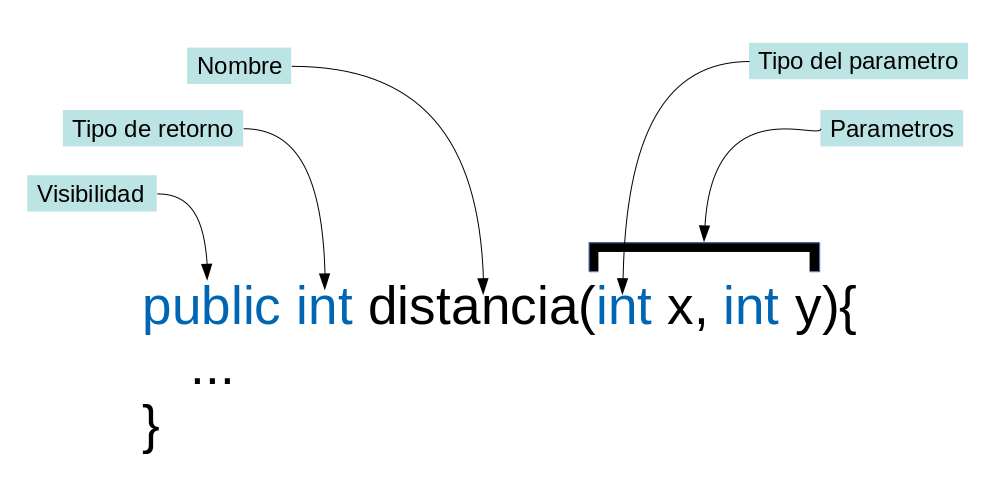
\includegraphics[width=12cm]{Firma.png}
\end{frame}

\begin{frame}
\frametitle{M\'etodo constructor}
\begin{itemize}
    \item Metodo encargado de colocar a un objeto en su estado inicial.
    \item Solamente es llamado cuando un objeto nevo es creado.
    \item Puede ser publico o privado.
    \item Se declara mediante el nombre de la clase.
    \item Se llama mediante la palabra reservada \emph{new}.
\end{itemize}
\end{frame}

\end{document}